\documentclass[a4paper, 12pt]{article}		% general format

%%%% Charset
\usepackage{cmap}							% make PDF files searchable and copyable
\usepackage[utf8x]{inputenc}				% accept different input encodings
\usepackage[T2A]{fontenc}					% Russian font
\usepackage[russian]{babel}					% multilingual support (T2A)

%%%% Graphics
\usepackage[dvipsnames]{xcolor}			% driver-independent color extensions
\usepackage{graphicx}						% enhanced support for graphics
\usepackage{wrapfig}						% produces figures which text can flow around

%%%% Math
\usepackage{amsmath}						% American Mathematical Society (AMS) math facilities
\usepackage{amsfonts}						% fonts from the AMS
\usepackage{amssymb}						% additional math symbols

%%%% Typography (don't forget about cm-super)
\usepackage{microtype}						% subliminal refinements towards typographical perfection
\linespread{1.3}							% line spacing
\usepackage[left=2.5cm, right=1.5cm, top=2.5cm, bottom=2.5cm]{geometry}
\setlength{\parindent}{0pt}					% we don't want any paragraph indentation
\usepackage{parskip}						% add distance between paragraphs

%%%% Tables
\usepackage{tabularx}						% Normal tables
\usepackage{multirow}						% for tabular
\usepackage{hhline}							% for tabular


%%%% Other
\usepackage{url}							% verbatim with URL-sensitive line breaks
\usepackage{fancyvrb}						% verbatim with box
\setcounter{secnumdepth}{5}					%

%------------------------------------------------------------------------------
\usepackage{listings}						% typeset source code listings

% Настройки отображения кода
\lstset{
	% Настройки отображения
	breaklines=true,						% Перенос длинных строк
	basicstyle=\ttfamily\footnotesize,		% Шрифт для отображения кода
	frame=tblr								% draw a frame at all sides of the code block
	tabsize=2,								% tab space width
	showstringspaces=false,					% don't mark spaces in strings
	% Настройка отображения номеров строк. Если не нужно, то удалите весь блок
	numbers=left,							% Слева отображаются номера строк
	stepnumber=1,							% Каждую строку нумеровать
	numbersep=5pt,							% Отступ от кода
	numberstyle=\small\color{black},		% Стиль написания номеров строк
}

% Для настройки заголовка кода
\usepackage{caption}
\renewcommand{\lstlistingname}{Листинг} % Переименование Listings в нужное именование структуры
%------------------------------------------------------------------------------
\author{Семён Мартынов\\<semen.martynov@gmail.com>}
\title{Отчет по лабораторной работе 4:\\SSL WebGoat}
\begin{document}
\maketitle
\tableofcontents{}

%------------------------------------------------------------------------------

\newpage
\section{Тестирование корректности настройки SSL}

\subsection{Цель работы}

Изучить сервис тестирования корректности настройки SSL на сервере Qualys SSL Labs -- SSL Server Test

\subsection{Ход работы}

Для изучения, рассмотрим сайт кафедры (kspt.icc.spbstu.ru) и его сертификат.

Первое, что обращает на себя внимание - это самоподписанный сертификат. И сервер выдаёт стандартную страницу Apache 2. Звёздочка на месте favicon даёт основание полагать, что сервер работает на Mandriva Linux (компания Mandriva на днях объявила о своём закрытии). Заголовок HTTP подтверждает эти догадки -- Apache/2.2.22 (Mandriva Linux/PREFORK-0.1mdv2010.2)

Дальнейшее изучение сертификата (см. рис. 2) показало неправильно выставленное значение поля CN и давно истекший срок валидности. В качестве алгоритма шифрования используется SHA-1, который браузер помечает как слабый, и предупреждает о прекращении поддержки таких сертификатов с 2017-го года.

\begin{figure}[h!]
\centering
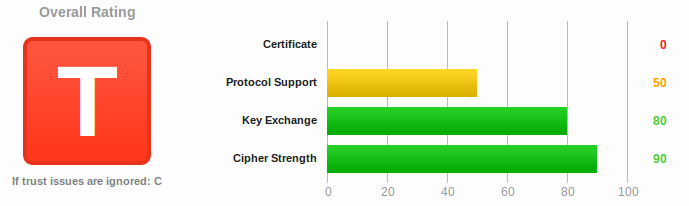
\includegraphics[scale=0.8]{res/pic002}
\caption{Анализ сертификата}
\end{figure}

На ошибку в CN обращает внимание и ssllabs.com. Но если проигнорировать все проблемы, связанные с тем, что это самоподписанный сертификат, результат достаточно не плохой -- ssllabs.com присвоил сертификату рейтинг C (см. рис. 1))

\begin{figure}[h!]
\centering
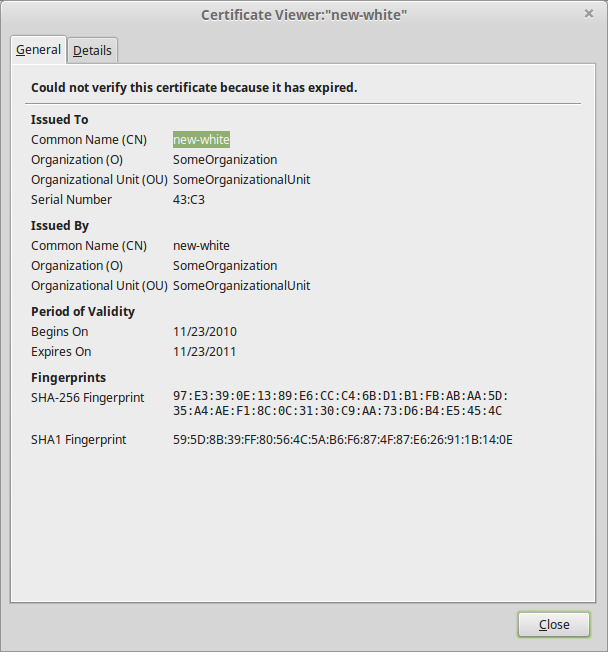
\includegraphics[scale=0.8]{res/pic001}
\caption{Сертификат kspt.icc.spbstu.ru}
\end{figure}

\subsubsection{Интерпретировать результаты в разделе Summary}

\paragraph{This server supports weak Diffie-Hellman (DH) key exchange parameters.}

Это показатель уязвимости под названием Logjam (обнаружена в различных реализациях протокола TLS). Уязвимость относится к типу \textit{downgrade} и позволяет клиенту понизить стойкость шифрования до 512 бит DH при условии поддержки сервером шифра DHE\_EXPORT, который задается в процессе рукопожатия (\textit{handshake}) между клиентом и сервером. Т. о. атакующему значительно проще организовать атаку типа Man-in-the-Middle (MitM). Уязвимость затрагивает как серверное ПО, использующее OpenSSL, и веб-браузеры.

\paragraph{This server is vulnerable to the POODLE attack.}

Знаменитая POODLE атака, вогнавшая последний гвоздь в SSL3. По причине того, что в SSLv3 padding не учитывается в MAC, злоумышленник может расшифровывать по 1 байту за 256 запросов, отправляя свои данные на сервер по SSLv3 от имени жертвы. Лечится полным отключением SSL3.

\paragraph{Certificate uses a weak signature. When renewing, ensure you upgrade to SHA2.} Как говорилось выше, поддержка SHA1 постепенно завершается. Здесь содержится рекомендация использовать SHA2 при следующем обновлении сертификата. 

\paragraph{The server supports only older protocols, but not the current best TLS 1.2.} Наиболее актуальной версией TLS на данный момент является версия 1.2, которая не поддерживается сервером.

\paragraph{The server private key is not strong enough.} В 2010-м году была представлена аккуратная реализация атаки на RSA1024 на основе ошибок железа.

\paragraph{This server accepts the RC4 cipher, which is weak.} В 2013-м году была представлена техника взлома Transport Layer Security и Secure Sockets Layer, если в них используется шифр RC4. Уязвимость RC4 связана с недостаточной случайностью потока битов, которым скремблируется сообщение. Прогоняя через него одно сообщение много раз, удалось выявить достаточное количество повторяющихся паттернов для восстановления исходного сообщения.

\paragraph{The server does not support Forward Secrecy with the reference browsers.} Сервер должен обеспечить гарантии того, что сессионные ключи, полученные при помощи набора ключей долговременного пользования, не будут скомпрометированы при компрометации одного из долговременных ключей.

\subsubsection{Расшифровать все аббревиатуры шифров в разделе Configuration}

\paragraph{TLS} -- Transport Layer Security.

\paragraph{SSL} -- Secure Sockets Layer.

\paragraph{RSA} -- аббревиатура от фамилий Rivest, Shamir и Adleman.

\paragraph{RC4} -- \textbf{R}ivest \textbf{c}ipher 4 или \textbf{R}on’s \textbf{c}ode 4.

\paragraph{SHA} -- Secure Hash Algorithm.

\paragraph{AES} -- Advanced Encryption Standard.

\paragraph{CBC} -- Cipher Block Chaining.

\paragraph{3DES} -- Triple Data Encryption Standard.

\paragraph{SNI} -- Server Name Indication

\paragraph{NPN} -- Next Protocol Negotiation.

\paragraph{HSTS} -- HTTP Strict Transport Security.

\paragraph{HPKP} -- HTTP Public Key Pinning.

\paragraph{HTTP} -- HyperText Transfer Protocol.

\subsubsection{Прокомментировать большинство позиций в разделе Protocol Details}

\paragraph{Secure Renegotiation} -- возобновление подключения TLS.

\paragraph{BEAST attack} --  атака утилитой BEAST (Browser Exploit Against SSL/TLS).

\paragraph{POODLE} -- уязвимость, позволяющая расшифровать содержимое защищённого канала коммуникации.

\paragraph{Downgrade attack} -- атака, при которой пользователя вынуждают использовать менее безопасные протоколы, которые всё ещё поддерживаются из соображений совместимости.

\paragraph{TLS compression} -- В 2012 году CRIME attack показал, как TLS сжатие может быть использовано злоумышленниками для выявления деталей конфиденциальных данных (например, сессионные куки).

\paragraph{Heartbleed} -- ошибка в OpenSSL, позволяющая несанкционированно читать память на сервере до 64 килобайт за один запрос. Атаку можно производить бесконечное количество раз.

\paragraph{Forward Secrecy} -- особенность протокола, который обеспечивает безопасный обмен данными, он не зависит от закрытого ключа сервера. С алгоритмами шифрования, которые не поддерживают Forward Secrecy, возможно расшифровать ранее зашифрованные разговоры с помощью закрытого ключа сервера.

\paragraph{Next Protocol Negotiation} -- клиент сообщает серверу по каким протоколам он бы хотел общаться и сервер может ответить наиболее предпочтительным из тех, которые он знает.

\paragraph{Strict Transport Security} -- механизм, активирующий форсированное защищённое соединение по HTTPS. Данная политика безопасности позволяет сразу же устанавливать безопасное соединение, вместо использования HTTP. Механизм использует особый заголовок HTTP Strict-Transport-Security, для переключения пользователя, зашедшего по HTTP, на HTTPS-сервер.

\subsection{Выводы}

На заданном сервере использовались механизмы генерации, заданные по умолчанию, т.е. системный администратор ничего сам не конфигурировал. Данный сертификат защищает пустую страницу, т.е. реальной опасности нет, но при использовании этого сертификата на продакшен-сервере наибольшую опасность представлял бы пудель.

%------------------------------------------------------------------------------

\newpage
\section{Проект OWASP WebGoat}

\subsection{Цель работы}

Изучить наиболее распространенные веб-уязвимости и познакомиться с OWASP WebGoat.

\subsection{Ход работы}

\subsubsection{Недостатки контроля доступа}

\subsubsection{Безопасность AJAX}

\subsubsection{Недостатки аутентификации}

\subsubsection{Переполнение буфера}

\subsubsection{Качество кода}

\subsubsection{Многопоточность}

\subsubsection{Межсайтовое выполнение сценариев}

\subsubsection{Неправильная обработка ошибок}

\subsubsection{Недостатки приводящие к осуществлению инъекций (SQL и прочее)}

\subsubsection{Отказ в обслуживании}

\subsubsection{Небезопасное сетевое взаимодействие}

\subsubsection{Небезопасная конфигурация}

\subsubsection{Небезопасное хранилище}

\subsubsection{Исполнение злонамеренного кода}

\subsubsection{Подделка параметров}

\subsubsection{Недостатки управление сессией}

\subsubsection{Безопасность веб-сервисов}

\subsection{Выводы}

%------------------------------------------------------------------------------

\end{document}
